% Součást skript na Datové struktury. Viz main.tex
\markright{$ $Id$ $}
% přepsal Vladimír Kotal

\chapter{Dynamizace}

V~uspořádaném poli umíme rychle vyhledávat, ale přidat prvky znamená
celé ho přebudovat. Ve~srůstajícím hašování zase nešly prvky mazat,
ve~velmi komprimovaných trie ani přidávat, ani mazat. V~této kapitole
ukážeme obecnou metodu, jak tyto problémy řešit, podobnou přístupu u
binomiálních hald.
\par
Takové struktuře, která neumožňuje vkládání (operace INSERT) ani mazání 
(operace DELETE) prvků budeme říkat
\emph{statická struktura}. Chceme vytvořit takovou reprezentaci, která
bude využívat výhod statické struktury, ale zároveň umožní operace INSERT
a DELETE.
\par
K tomu se dopracujeme postupně. 
Nejdříve provedeme \emph{semidynamizaci}, 
která umožní (v nové reprezentaci původní množiny) operaci INSERT, 
pak \emph{dynamizaci}, která přidá operaci DELETE. 



% --------------------------------------------------------------------------
\section{Zobecněný vyhledávací problém}

\begin{defn}
\emph{Vyhledávací problém} je funkce $f: U_1 \times 2^{U_2} \to U_3$, kde
$U_1$, $U_2$ a $U_3$ jsou univerza.
\end{defn}
\begin{defn}
\emph{Řešení vyhledávacího problému} pro $x \in U_1, A \subseteq U_2$
je nalezení hodnoty $f(x, A)$.
\end{defn}

\begin{pozn}
Chceme najít strukturu, která reprezentuje A a algoritmus, který pro vstup
$x \in U_1$ spočítá $f(x, A)$. Takové struktuře se říká 
\emph{statická struktura} pro vyhledávací problém.
\end{pozn}

\begin{priklad}
\begin{description}
\item[Klasický vyhledávací problém:]
	
	$U_1 = U_2 = U$, univerzum prvků; \\
	$U_3 = \{0, 1\}, A \subseteq U_2$ 

	$f(x, A) =
	\begin{cases}
	0& \text{když } x \notin A\\
	1& \text{když } x \in A
	\end{cases}$
	(rozložitelný)
\item[Euklidovská vzdálenost bodů v rovině:]

	$U_1 = U_2 = $ euklidovská rovina; 
	$U_3 = \mathbb{R}^+$; 
	$f(x, A) = dist(x,A$ vzdálenost bodu $x \in U_1$ od množiny $A$.
	(rozložitelný, $\oplus$ ... operace min)
\item{Nalezení předchůdce}
	$U_1 = U_2 = U_3$ 
	pro $x \in U_1$ a $A \subseteq U_!$ a je $f(x,U_!)$ je největší 
		prvek $A \leq x$
	(rozložitelný, je potřeba disjunkce)
\item[Příslušnost ke konvexnímu obalu]

	$U_1 = U_2 = $ rovina; 
	$U_3 = \{0, 1\}$;

	\begin{figure}[!htb]
	\centering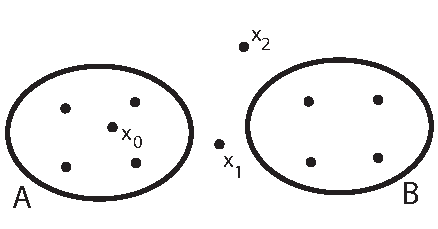
\includegraphics{pics/convex-envel}
	\caption{Konvexní obal}
	\label{convex-envel}
	\end{figure}

	\(f(x, A) =
	\begin{cases}
	0& \text{když $x$ nepatří do konvexního obalu $A$}\\
	1& \text{když $x$ patří do konvexního obalu $A$}
	\end{cases}\)
	(není rozložitelný problém)
\end{description}
\end{priklad}


\subsection{Operace INSERT a DELETE}

Pro množinu $A \subseteq U_2$ a pro statickou strukturu {\cal S}
řešící vyhledávací problémf pro $x \in U_2$.
\par
\begin{itemize}
\item INSERT($x$,$A$) - vybudování struktury řešící vyhledávací problém pro množinu
$A \cup \{x\}$
\item DELETE($x$,$A$) - vytvoření struktury řešící vyhl. problém pro množinu 
$A - \{x\}$
\end{itemize}

\begin{pozn}
Ze statické struktury chce vytovořit dynamickou (dynamizace). INSERT je
obvykle jednodušší než DELETE, na ten budeme potřebovat dodatečné
předpoklady.
\end{pozn}

Nároky na dynamizaci
\begin{itemize}
\item chceme aby se $f(x,A)$ v nové struktuře spočítalo přibližně 
  stejně rychle jako v původní struktuře
\item když vytvoření původní struktury pro $n$ prvnkovou množinu trvalo
  $t$, pak operace INSERT by přibližně měla vyžadovat čas $t/n$.
\end{itemize}

\begin{defn}
Vyhledávací problém je \emph{rozložitelný}, když
existuje operace $\oplus$ spočitatelná v konstantním čase a platí:
když $x \in U_1$ a $A$ a $B$ jsou disjunktní podmnožiny $U_2$, pak
\[
	f(x, A \cup B) = f(x, A) \oplus f(x, B).
\]
\end{defn}

\begin{pozn}
Z výše uvedených příkladů není rozložitelným problémem příslušnost ke
konvexnímu obalu, ostatní vyhledávací problémy jsou rozložitelné.
\end{pozn}

\newcommand{\staticka }{\ensuremath{\mathcal{S}}}
\newcommand{\dynamicka}{\ensuremath{\mathcal{D}}}


\begin{defn}
Nechť $f$ je rozložitelný vyhledávací problém a $\staticka$ je
``statická'' datová struktura, která ho řeší. Neboli $\staticka$ je
tvořena pro pevnou množinu $A \subseteq U_2$ a obsahuje operaci, která
pro vstup $x$ počítá $f(x, A)$.

Popíšeme důležité parametry $\staticka$: nechť $n = |A|$, označme
\begin{align*}
Q_\staticka(n) & = \text{čas potřebný pro výpočet $f(x,A)$}\\
S_\staticka(n) & = \text{paměť potřebná pro vybudování \staticka}\\
P_\staticka(n) & = \text{čas potřebný pro vybudování \staticka}
\end{align*}
\end{defn}

% ------------------------------------------------------------------------
\section{Semi-dynamizace}

Semi-dynamizace umožní operaci INSERT nad novou reprezentací původní
množiny. Tato reprezentace bude využívat statické struktury. Nejprve
provedeme "základní" semidynamizaci, poté ji vylepšíme pro INSERT se
složitostí v nejhorším případě. Vylepšení bude vyžadovat jiný rozklad
původní množiny a algoritmus INSERT (viz
algoritmus~\ref{alg:semidyn.insert.vylepseny}) 
bude složitější.

\begin{theorem}
Máme rozložitelný vyhled. problém $f$ a máme pro něj statickou strukturu,
která ho řeší v čase $Q(n)$, vyžaduje $S(n)$ paměti a vytvoří se v čase
$P(n)$,
kde $Q(n), \frac{P(n)}{n}, \frac{S(n)}{n}$ jsou neklesající funkce. Pak
existuje semidynamická dat. struktura $D$, řešící $f$ v čase
$O(Q(n)\log n)$ vyžadující $O(S(n))$ paměti a umožňující INSERT s 
amort. složitostí
$O(\frac{P(n)}{n} \cdot\log n)$.
\end{theorem}

\begin{proof}
Budeme předpokládat, že $Q_\staticka(n)$, $S_\staticka(n)/n$ a
$P_\staticka(n)/n$ jsou neklesající funkce.

Máme množinu $A$ a vytvoříme pro ni novou strukturu $D$.
Nechť $A_i \subseteq A$ taková, že buď $|A_i| = 2^i$ nebo $A_i = \emptyset$ \\
$A_i \cap A_j = \emptyset {\text pro } i \neq j$.
$\bigcup A_i = A$

Platí $A_i \neq \emptyset$ právě když $(i+1)$-ní bit v dvojkovém rozvoji čísla
$|A|$ je 1.

Chceme navrhnout strukturu, která by uměla
\begin{enumerate}
\item Pro $x \in U_1$ a pevné $A \subseteq U_2$ rychle spočítat $f(x, A)$.
\item Pro $A$ a $y \in U_2$ rychle vytvořit strukturu pro $A \cup \{y\}$.
\end{enumerate}

Mějme $A_0, A_1, \cdots$ takové, že
\begin{enumerate}
\item $A_i \cap A_j = \emptyset$ pro $i \neq j$
\item buď $A_i = \emptyset$ nebo $|A_i| = 2^i$ 
\item $\bigcup_i A_i = A$ 
\end{enumerate}

Nová struktura \dynamicka\ reprezentující $A$ je potom
\begin{itemize}
% \item XXX Seznam statických struktur pro $A_i \neq \emptyset$, $\staticka_i$
\item nějaká dynamická struktura reprezentující A
(např. (a,b)-strom, červeno-černý strom, AVL-strom)
% \item XXX Vyhledávací strom reprezentující $A$
\item Pro každé $A_i \neq \emptyset$ máme S strukturu reprezentující $A_i$.
\item Pro každé $A_i \neq \emptyset$ seznam prvků v $A_i$; prvky
těchto seznamů jsou projpojeny s odpovídajícími prvky ve stromě.
\end{itemize}

Jak v nové struktuře spočítáme $f(x,A)$ ? \\
Pro každou $A_i \neq \emptyset$ spočítáme $f(x,A_i)$ a pomocí operace
$\oplus$ pak spočítáme $f(x,A)$.

\begin{pozn}
Platí, že když $A_i \neq \emptyset$, pak 
$i \leq \lceil log_2|A| \rceil$
\mnote{XXX jak ma vypadat tento vzorec ?}
čas, který je potřeba v nové struktuře na výpočet $f(x,A)$
\end{pozn}

\begin{multline}
log_2|A| + \sum_{i=0}^{log|A|}Q(2^i) \leq log|A| + \sum_{i=0}^{log|A|}Q(|A|)
= log|A|(Q(|A|) + 1)
\end{multline}

\begin{pozn}
První nerovnost plyne z toho, že $Q(n)$ je nerostoucí funkce. 
V dalších důkazech pro $S$ a $P$ se využívá opět této vlastnosti pro
$\frac{S(n)}{n}$ a $\frac{P(n)}{n}$.
\end{pozn}

$log_2(|A|)$ - vyhodnocení $f(x,A)$ z $f(x,A_i), i=0,1,...$
\par

Tedy algoritmus potřebuje $O(log|A| Q(|A|))$ času
když $Q(n) = \Theta(n^\epsilon) pro \epsilon > 0$, pak platí, že nová
struktura pro výpočet $f$ potřebuje
\begin{equation}
\begin{split}
& log|A| + \sum_{i=0}^{log n}Q(2^i)  \\
& = |A| + \sum_{i=0}^{log |A|}
\frac{S(2^i)}{2^i} 2^i \leq |A| + \sum_{i=0}^{log |A|} \frac{S(|A|)}{|A|} 2^i \\
& = |A| - \frac{S(|A|)}{|A|} 2^i = |A| -
\frac{S(|A|)}{|A|}(\sum_{i=0}^{log |A|} 2^i) \\
& = O(S(|A|))
\end{split}
\end{equation}

\subsection{INSERT}


\begin{algorithm}[!htb]
\caption{INSERT pro semidynamizaci (rozklad $A$ na množiny $A_i$)}
\label{alg:semidyn.insert}
\begin{algorithmic}
\STATE INSERT(x)
\IF {$x \not\in A$} 
  \STATE nalezneme nejmenší $j$, že $A_j = \emptyset$
\ENDIF
\STATE $A_j = \{x\} \cup \bigcup{i<j} A_i, A_i = \emptyset$ pro $i<j$
\STATE vytvoříme strukturu $S$ spojový seznam pro $A_j$
\STATE $x$ přidáme do reprezentace $A$.
\end{algorithmic}
\end{algorithm}


Kdy se buduje znovu (tedy podruhé) $S$ struktura pro $A_j$ (měřeno počtem
INSERTů) ?
\begin{enumerate}
\item musí se naplnit všechny $A_i$ pro i<j 
to je $2^j-1$ úspěšných INSERTů (ty, které přidaly prvek)
\item provede se úspěšný INSERT, který vyprázdní $A_i$ pro $i \leq j$
\item znovu se musí naplnit $A_i$ tj. $2^j-1$ úspěšných INSERTů
\item daší úspešný INSERT vytvoří teprve S strukturu pro $A_j$
\end{enumerate}

tj. $2^j -1 + 1 + 2^j -1 + 1 = 2 \cdot 2^j = 2^{j+1}$ úspěšných INSERTů.

Amortizovaný čas operace INSERT je 
$$
log |A| + \sum_{i=0}^{log |A|} \frac{P(2^j)}{2^{j+1}} \leq
log |A| + \sum_{i=0}^{log |A|} \frac{P|A|}{|A|} = 
O(log |A| \cdot \frac{P|A|}{|A|})
$$

\end{proof}

\begin{theorem}
Máme rozložitelný vyhledávací problém $f$ a máme pro něj statickou strukturu,
která ho řeší v čase $Q(n)$, vyžaduje $S(n)$ paměti a vytvoří se v čase
$P(n)$,
$kde Q(n), \frac{P(n)}{n}, \frac{S(n)}{n}$ jsou neklesající funkce. Pak
existuje semidynamická dat. struktura $D$, řešící $f$ v čase
$O(Q(n)\log n)$ vyžadující $O(S(n))$ paměti a umožňující INSERT se
složitostí
$O(\frac{P(n)}{n} \cdot\log n)$.
\end{theorem}

% ------------------------------------------------------------------------

\subsection{INSERT se složitostí v nejhorším případě}

Následuje konstrukce takové semidynamické struktury, která bude podporovat
INSERT se složitostí v nejhorším případě.

\begin{pozn}
Pokud $\frac{P(n)}{n} = \Theta(n^\varepsilon)$ pro $\varepsilon > 0$, pak
amortizovaný čas pro operaci INSERT bude $O(\frac{P|A|}{|A|})$.
\end{pozn}

Máme množinu $A$ \\
budeme mít roklad $A$ na disjunktní množiny $A_{i,j}, i=0,1,..., j \in
{0,1,...,k_j}$, kde $k_j \in {0,1,2}$. \\
$|A_{i,j}| = 2^i$ a platí: \\
když $A_{i,0}$ existuje pro $i > 0$, pak existují $A_{i-1,0}, A_{i-1,1}$.
\par

Struktura: 
\begin{enumerate}
\item reprezentace $A$ (pomocí (a,b)-stromů, červeno-černých stromů, ...)
\item $\forall$ existující $A_{i,j}$ je $S$ struktura reprezentující
$A_{i,j}$ 
\item $\forall$ existující $A_{i,j}$ je spojový seznam reprezentující
$A_{i,j}$
\item když $A_{i,0}$ a $A_{i,1}$ existují pro nějaké i, pak je 
"rozpracovaná" $S$ struktura pro množinu $A_{i-1,k_i+1} = A{i,0} \cup
A_{i,1}$.
tj. bylo provedeno několik kroků pro její vytvoření, ale není dokončena.
\end{enumerate}


% nasleduje prednaska z 12.5.2003, prepsal Vladimír Kotal


$A \subseteq U_2, i_0 \in N$ \\
$\forall i = 0,1,...,i_0$ je dáno $j_i \in {0,1,2}$ takové, že $j_i > 0$
když $i < i_0$. \\
$\forall i = 0,1,...,i_0$ a $\forall j = 0,1,...,j_i$ je $A_{i,j} \in A$
taková, že $|A_{i,j}| < 2^i$.

\begin{defn}
${ A_{i,j}, i=0,1,...,i_0, j=1,2,...,j_i }$ je rozklad $A$.
\end{defn}

Pro každé $A_{i,j}$ je dána $S$ struktura reprezentující $A_{i,j}$ a spojový
seznam prvků z $A_{i,j}$, navíc dána dat. struktura reprezentující A.
Když $A_{i,1}$ existuje, pak je rozpracovaná S struktura pro
$A_{i+1,j_{i+1}+1} = A_{1,0} \cup A_{i,1}$.

\begin{pozn}
Struktura je rozpracovaná, jestliže bylo provedeno několik kroků
pro postaverní $S$ struktury, ale ještě není dokončena.
\end{pozn}

- toto je definice nové semidynamické struktury.

Paměťové nároky
\begin{equation}
\begin{split}
& |A| + \sum_{i=0}^{log |A|} 4S(2^i) \\
& = |A| + \sum_{i=0}^{log |A|} \frac{S(2^i)}{2^i}2^i \leq 
|A| + 4 \sum_{i=0}^{log |A|} \frac{S(|A|)}{|A|}2^i \\
& = |A| + \frac{4S(|A|)}{|A|} (\sum 2^i) = |A| + 4S(|A|) \\
& = O(S(|A|))
\end{split}
\end{equation}

\begin{pozn}
$|A|$ - paměť pro pom. struktury  \\
$\sum_{i=0}^{log |A|} 4S(2^i)$ - paměť potřebná na S struktury
\end{pozn}

Algoritmus pro výpočet : \\
spočítáme $f(x,A_{i,j})$ pro každou $A_{i,j}$ a pomocí operace $\oplus$
spočítáme $f(x,A)$. 

Čas potřebný pro výpočet $A$
\begin{multline}
\sum_{i=0}^{log |A|} 3Q(2^i) + 3\log |A| \leq 
3\sum_{i=0}^{log |A|} Q(|A|) + 3\log |A| = 
3Q(|A|)log |A| = O(Q(|A|)\log |A|)
\end{multline}

Platí: $Q(n) \geq n^{\epsilon}$ pro nějaké $\epsilon$, pak čas potřebný pro
výpočet $f$ je $O(Q(N))$.

INSERT(x) viz alg.~\ref{alg:semidyn.insert}

%\begin{algorithm}[!htb]
%\caption{Operace INSERT pro semidynamizaci}
%\label{alg:semidy.insert}
%\begin{algorithmic}
%\STATE když $x \notin A$ jinak provedeme:
%  \STATE vytvoříme S strukturu pro $A_{0,j_i+1} = \{x\}$ (zvětšíme $j_0$ o 1)
%  \IF {$j_o$ je liché}
%      \STATE pak provedeme 1.krok pro vytvoření S struktury
%      \STATE pro množinu $A_{1,j_1 + \lceil \frac{j_0}{2} \rceil} = A_{0,j_0 - 1}
%      \cup A_{0,j_0}$
%  \ENDIF
%  \STATE pro $i = 1,2,...,i_0+1$ v roustoucím pořadí:
%  \IF {S je rozpracovaná struktura pro $A_{i,j_i+1}$}
%    \STATE provedeme dalších $\frac{P(2^i)}{2^i}$ kroků pro její vybudování
%  \ENDIF
%  \STATE když jsme dobudovali S strukturu pro $A_{i,j_i+1}$, zvětšíme $j_i$ o 1
%  \STATE zrušíme $A_{i-1,0} \cup A_{i-1,1}$, zmenšíme $j_i$ o 2 a $A_{i-1,j}$ přepíšeme
%  na $A_{i-1,j_i+2}$.
%  \IF {$j_i$ liché} 
%    \STATE provedeme 1.krok pro vytvoření Q struktury pro
%    \STATE množinu $A_{1,j_i+1 + \lceil \frac{j_i}{2}} = A_{i,j_i} \cup A_{i,j_i-1}$.
%  \ENDIF
%\end{algorithmic}
%\end{algorithm}


\begin{algorithm}[!htb]
\caption{INSERT pro semidynamizaci (rozklad $A$ na $A_{i,j}$)}
\label{alg:semidyn.insert.vylepseny}
\begin{algorithmic}
\STATE INSERT(x)
\IF{$x \not\in A$}
  \STATE postavíme S-strukturu pro množinu $A_{0,j_0}={x}$
  \STATE $j_0$++
  \STATE $i=1$
  \WHILE{$j[i]>0$} 
    \IF{S-struktura pro $A_{i,j_i-1}$ není dostavěna}
      \STATE provedeme dalších $P(2^i)/2^i$ kroků pro vystavění 
      	S-stry pro $A_{i,j_i-1}$
      \IF{S-stra pro $A_{i,j_i-1}$ je dostavěna}
        \STATE $A_{i-1,0}=A_{i-1,2}$
        \STATE $A_{i-1,1}=A_{i-1,3}$
        \IF{$i-1>0$} 
          \STATE // na všech úrovních kromě 0-té, dojde k tom, že $j_i=5$
	  \STATE // tj. S-struktura pro $A_{i,4}$ je rozestavěna
          \STATE // poprvé k tomu dojde při 10. INSERTu, takže trpělivost
	  \STATE $A_{i-1,2}=A_{i-1,4}$
	\ENDIF
        \STATE $j_{i-1}=j_{i-1}-2$
        \STATE $A_{i,j_i}=A_{i-1,0} + A_{i-1,1}$
        \STATE provedeme první krok pro vystavění S-stry pro A[i,j[i]]
        \STATE $j_i$++
      \ENDIF
    \ENDIF
    \STATE $i++$
  \ENDWHILE

  \IF{$j[i-1] > 1$ a S-struktury pro $A_{i-1,0}$ a $A_{i-1,1}$ jsou dostavěny}
    \STATE $A_{i,0}=A_{i-1,0} + A_{i-1,1}$
    \STATE provedeme první krok pro vystavění S-struktury pro $A_{i,0}$
    \STATE $j_i$++
  \ENDIF
\ENDIF
\end{algorithmic}
\end{algorithm}

\mnote{Alg. INSERT pro semidyn. byl ověřen doktorem Koubkem}

\begin{pozn}
Může stát, že se vytvoří nová množina $A[i,j(i)]$, pak $j(i)$ má hodnotu
5, tj. musí se po dokončení struktury $A[i+1,j(i+1)-1]$ zmenšit o dvě
hodnoty $A(i,2)$, $A(i,3)$ a i $A(i,4)$ (nestačí jen pro první dvě hodnoty).
\end{pozn}

Čas pro INSERT(x) je \\
\begin{multline}
log |A| + \sum_{i=0}^{log |A|} (\frac{P(2^i)}{2^i} + 1) = 
2log |A| + \sum_{i=0}^{log |A|} \frac{2P(|A|)}{|A|} = \\
2log |A| + \frac{2P(|A|)}{|A|} \sum_{i=0}^{log |A|} 1 = 
2log |A| \frac{2P(|A|)}{|A|} log |A| = O(\frac{2P(|A|)}{|A|} log |A|)
\end{multline}

$log |A|$ - čas pro zjištění zda $x \in A$ \\

Když $\frac{P(n)}{n} \geq n^{\varepsilon}$ pro $\varepsilon > 0$, pak INSERT
vyžaduje čas $O(\frac{P(n)}{n})$.

\par
\begin{priklad}
XXX
\par
\vspace{5mm}

\begin{tabular}{|l|l|l|}
\hline
INSERT($x_1$) & INSERT($x_2$) & INSERT($x_3$) \\
\hline
$A_{0,0} = \{x_1\}$ & $A_{0,0} = \{x_1\}$ & $A_{0,0} = \{x_1\}$ \\
 & $A_{0,1} = \{x_2\}$ & $A_{0,1} = \{x_2\}$ \\
 & 1. krok pro $A_{1,0} = \{x_1,x_2\}$ & $A_{0,2} = \{x_3\}$ \\
 & & $\frac{P(2)}{2}$ kroků pro $A_{1,0} = \{x_1,x_2\}$ \\
 % \vspace{1mm}
\hline
INSERT($x_4$) & INSERT($x_5$) & INSERT($x_6$) \\
\hline
% XXX prvni dva radky skrtneme 
% prepsat skrtani poradne ze zapisku
$A_{0,0} = \{x_1\}$ & $A_{0,0} = \{x_3\}$ & $A_{0,0} = \{x_3\}$ \\
$A_{0,1} = \{x_2\}$ & $A_{0,1} = \{x_4\}$ & $A_{0,1} = \{x_4\}$ \\
$A_{0,2} = \{x_3\} \rightarrow A_{0,0} = \{x_3\}$ &
$A_{0,2} = \{x_5\}$ &
$A_{0,2} = \{x_5\} \rightarrow A_{0,0} = \{x_5\}$ \\
$A_{0,3} = \{x_4\} \rightarrow A_{0,1} = \{x_4\}$ &
$A_{1,0} = \{x_1,x_2\}$ &
$A_{0,3} = \{x_6\} \rightarrow A_{0,1} = \{x_6\}$ \\
dokončíme $A_{1,0} = \{x_1,x_2\}$ &
$\frac{P(2)}{2}$ kroků pro $A_{1,1} = \{x_3,x_4\}$ &
$A_{1,0} = \{x_1,x_2\}$ \\
1. krok pro $A_{1,1} = \{x_3,x_4\}$ & &
dokončeno $A_{1,1} = \{x_3,x_4\}$ \\
& & 1. krok pro $A_{1,2} = \{x_5,x_6\}$  \\
& & 1. krok pro $A_{2,0} = \{x_1,x_2,x_3,x_4\}$ \\
& & $\frac{P(4)}{4}$ kroků \\
% \vspace{1mm}
\hline
\end{tabular}

\end{priklad}

\begin{theorem}
Nechť $S$ je statická struktura pro rozložitelný vyhledávací problém $f$
a nechť $K$ je "hladká" funkce. Pak existuje semidynamická struktura $D$
založená na rozkladu určeném funkcí $K$, tak že platí: \\
když $K=O(log n)$, pak čas pro vyhledání je $O(K Q(n))$ \\
			  pro INSERT je $O(K(n) n^{\frac{1}{K(n)}}
			  \frac{P(n)}{n})$ \\
Když $K = \Omega(log(n))$, pak platí: \\
čas pro vyhledání je $O(K(n)) Q(n))$ \\
Pro INSERT je $O(\frac{log(n)}{log \frac{K(n)}{log(n)} }
\frac{P(n)}{n})$.
\end{theorem}

\begin{proof}
viz \cite{mehlhorn-overmars}.
\end{proof}

% dynamizace ----------------------------------------------------------

\section{Dynamizace}

Potřebujeme, aby struktura $S$ připouštěla falešný DELETE (prvek pouze
škrtneme, ale zůstane tam. falešný - čas. ani paměťové nároky se nezlepší
ani nezhorší)

\begin{defn}
\emph{Falešný DELETE} je operace, která vyškrtne prvek z množiny - tj. umožní
počítat $f(x,A-\{a\})$ (kde a je vyškrtnutý prvek) tak, že časové nároky
budou stejné jako když nebyl žádný prvek vyškrtnut.
\end{defn}

Budeme předpokládat, že čas pro falešný DELETE je $O(n)$, kde $n$ je velikost
původní reprezentované množiny.

\subsection{Reprezentace množiny A}

Rozložíme $A$ na disjunktní množiny $A_j, j=0,1,...,log|A|+3$
takové, že buď $A_j = \emptyset$ nebo $2^{j-3} < |A_j| \leq 2^j$.
\par
každá množina $A_j$ bude reprezentována strukturou, která původně (když
nebyly vyškrtnuté žádné prvky) měla velikost $\leq 2^j$.
\par
Dále $\forall A_j \neq \emptyset$ bude dán spojový seznam prvků v $A_j$.
\par
Bude dána datová reprezentace množiny $A$. Pro každý prvek a v spojovém
seznamu množiny $A_j$ bude dán ukazatel na prvek a  v dat. struktuře
reprezentující A a naopak. Pro každý prvek v dat. struktuře repr. $A$ je dán
ukazatel na prvek a v odpovídajícím spojovém seznamu.

\subsection{Paměťové nároky}

\begin{multline}
|A| + \sum_{i=0}^{log|A|+3} S(2^i) = |A| + \sum \frac{S(2^i)}{2^i} 2^i
\leq |A| + \sum_{i=0}^{log|A|+3} \frac{S(8|A|)}{8|A|} 2^i = \\
|A| + \frac{S(8|A|)}{8|A|} 2^i = |A| + \frac{S(8|A|)}{8|A|} \sum 2^i = 
|A| + S(8|A|) = O(S(8|A|))
\end{multline}
\par

$|A|$ - pomocné struktury \\
suma - paměť pro $S$ struktury
\par
Závěr: Když $S$ je omezená polynomem, pak paměťové nároky jsou $O(S(n))$.
Pokud $S$ je superpolynomiální, pak paměť. nároky jsou $O(S(8n))$
(a platí $S(n) = o(S(8n))$)
\par

Výpočet $f$: \\
spočítáme $f(x,A_j)$ a pomocí operace $\oplus$ spočítáme $f(x,A)$.

\subsection{Čas pro výpočet $f$}

$log(n) + \sum_{i=0}^{log|A|+3} Q(2^i) = log(n) + \sum Q(8|A|) =
O(Q(8|A|) log|A|)$.
\par

Závěr: čas na výpočet $f$ je
$\Biggl\{$
\begin{tabular}{ll}
když $Q$ je subpolynomiální & $O(Q(n)log(n))$ \\
polynomiální & $O(Q(n))$ \\
superplynomiální & $O(Q(8n))$ \\
\end{tabular}

% zde začíná poslední přednáška ze šk.r.2002/2003
% thanks to Jana Skotaková za zapůjčení, přepsal Vladimír Kotal

INSERT(x) viz alg. \ref{alg:dynam.insert_f}

\begin{algorithm}[!htb]
\caption{Operace INSERT (f)}
\label{alg:dynam.insert_f}
\begin{algorithmic}
\IF {$x \not \in A$}
  \STATE nalezneme nejmenší j takové, že $|\bigcup i \leq j A_i| < 2^j$
\STATE položíme $A_j = \bigcup{i\leq j}A_i \cup \{x\}$
\STATE $A_i = \emptyset pro i < j$
\STATE vytvoříme S-strukturu a spojový seznam pro $A_j$ (x přidáme do
struktury reprezentující A a přidáme požadované ukazatele)
\ENDIF  
\end{algorithmic}
\end{algorithm}

\par
Pozorování:\\
Když vytváříme při INSERTu S-strukturu pro $A_j$, pak $2^{j-1} < |A_j|
\leq 2^j$. \\
(když toto neplatí, pak pro $j-1$ je splněna nerovnost $|\bigcup{i<j-1} A_i|
< 2^{j-1}$ a to je spor s minimalitou $j$.
\par

% viz poznamky/datstr_054.jpg
DELETE(x) viz alg. \ref{alg:dynam.delete_f}

\begin{algorithm}[!htb]
\caption{Operace INSERT (f)}
\label{alg:dynam.delete_f}
\begin{algorithmic}
\IF {$x \not \in A$}
  \STATE odstraníme x ze struktury pro A
  \STATE nalezneme j takové, že $x \in A_j$ (budeme znát přímo místo x v seznamu
  pro $A_j$)
  \IF {$|A_j| = 1$}
    \STATE smažeme $A_j$ (odpovídající S-strukturu 
% tady to snad pokracuje     
     a spojový seznam) $\rightarrow A_j = \emptyset$
  \ENDIF
  \IF {$|A_j| > 1$ a zároveň $|A_j| > 2^{j-3} + 1$}
    \STATE na $S$ strukturu pro $A_j$ provedeme falešný DELETE($x$), $x$ smažeme
    ze spojového seznamu pro $A_j \rightarrow A_j = A_j - \{x\}$
  \ENDIF  
  \IF {$|A_j| > 1$ a zároveň $|A_j| = 2^{j-3} + 1$}
    \IF {$A_{j-1} = \emptyset$}
       \STATE $A_{j-1} = A_{j-1} - \{x\}, A_j = \emptyset$
       \STATE vybudujeme novou S-strukturu pro $A_{j-1}$
       ($x$ odstraníme ze spojového seznamu pro $A_{j-1} - 1$)
% \mnote{XXX tady nevím jestli nemá být jenom $A_{j-1}$}
    \ENDIF
    \IF {$A_{j-1} = \emptyset$ a zároveň $|A_{j-1}| > 2^{j-2}$}
      \STATE vyměním $A_j a A_{j-1}$
      \STATE z $A_{j-1}$ odstraníme x a vytvoříme novou S-strukturu pro
      $A_{j-1}$ (původní struktura mohla mít až $2^j$ prvků)
    \ENDIF
    \IF {$A_{j-1} = \emptyset$ a zároveň $|A_{j-1}| \leq 2^{j-2}$}
      \STATE $B = (A_j \cup A_{j-1}) - \{x\}$\
      \STATE zrušíme S-struktury pro $A_j, A_{j-1}$ a vybudujeme S-strukturu
      a spojový seznam pro B
      \IF {$|B| \geq 2^{j-2}$}
        \STATE $A_j = B, A_{j-1} = \emptyset$
      \ELSE
        \STATE $A_{j-1} = B, A_j = \emptyset$
      \ENDIF	
    \ENDIF
  \ENDIF
\ENDIF  
\end{algorithmic}
\end{algorithm}

Pozorování: \\
Když operace DELETE buduje $S$-strukturu pro množinu $A_j$, pak platí:
$2^{j-1} \leq |A_j| \leq 2^{j-1}$.

\subsection{Amortizovaný čas operace DELETE}

$$
(log|A| + D(2^j) + P(2^j) =
(log|A| + D(2^j) + \frac{P(2^j)}{2^{j-3}}) = O(log|A| + D(|A|) +
4\frac{P(|A|)}{|A|})
$$

\begin{itemize}
\item $log|A|$ - zjištění zda $x \in A$ 
\item $D(2^j)$ - falešný DELETE 
\item $\frac{P(2^j)}{2^{j-3}}$ - budování S-struktury pro $A_i$
\end{itemize}

Aby DELETE znovu vytvářel S-strukturu pro množinu v $A_i$, musím provést
aspoň $2^{j-3}$ operací DELETE.

\subsection{Amortizovaný čas operace INSERT}

Když INSERT vytvářel S-strukturu pro $A_i,$ pak $A_j = \emptyset$ pro
$j<i$ a aby se znovu vytvářela struktura pro $A_i$, musí platit:
$$
1 + \sum_{j \leq i}{} |A_j| > 2^{j-1}
$$

DELETE zaplní $A_j$ jen do poloviny. To znamená, že se musí provést alespoň
$2^{j-2}$ INSERTŮ, tedy amortizovaná složitost je
$$
O(log|A| + \sum_{}{} \frac{P(2^i)}{2^{i-2}}) = O(\frac{P(|A|)}{|A|} log n)
$$

Práce s pomocnými stukturami zabere práve $log|A|$ času.
\par
Když $P(n)=n^{\epsilon}$ pro $\epsilon > 0$, pak amortizovaná složitost je
$O(\frac{P(|A|)}{|A|})$.

% EOF
